\documentclass[UTF8,10pt,twocolumn,letterpaper]{article}
\usepackage[hyperref, UTF8]{ctex}
\usepackage{cvpr}
\usepackage{times}
\usepackage{epsfig}
\usepackage{graphicx}
\usepackage{amsmath}
\usepackage{amssymb}



% Include other packages here, before hyperref.

% If you comment hyperref and then uncomment it, you should delete
% egpaper.aux before re-running latex.  (Or just hit 'q' on the first latex
% run, let it finish, and you should be clear).
\usepackage[breaklinks=true,bookmarks=false]{hyperref}

\cvprfinalcopy % *** Uncomment this line for the final submission

\def\cvprPaperID{****} % *** Enter the CVPR Paper ID here
\def\httilde{\mbox{\tt\raisebox{-.5ex}{\symbol{126}}}}

% Pages are numbered in submission mode, and unnumbered in camera-ready
%\ifcvprfinal\pagestyle{empty}\fi
\setcounter{page}{4321}
\begin{document}

%%%%%%%%% TITLE
\title{微信跳一跳辅助}

\author{张子垚\\
\and
李宝伟\\
\and
何湛辉\\
}

\maketitle
%\thispagestyle{empty}

%%%%%%%%% ABSTRACT
\begin{abstract}
   2017 年 12 月 28 日下午,微信发布了 6.6.1 版本,加入了「小游戏」功能,并提供了官方 DEMO「跳一跳」。这是一个 2.5D 插画风
   格的益
   智游戏,玩家可以通过按压屏幕时间的长短来控制这个「小人」跳跃的距离。分数越高,那么在好友排行榜更加靠前。~\cite{Authors14}
   这次我们利用图像识别的技术,对跳一跳进行分析,从而有此辅助的诞生,仅供交流学习。
\end{abstract}

%%%%%%%%% BODY TEXT
\section{介绍}

每次落稳之后截图,根据截图算出棋子的坐标和下一个块顶面的中点坐标,根据两个点的距离乘以一个时间系数获得长按的时间。靠棋子的颜
色来识
别位置,通过截图发现最下面一行大概是一条直线,就从上往下一行一行遍历,比较颜色(颜色用了一个区间来比较)找到最下面的那一行的
所有
点,然后求个中点,求好之后再让 Y 轴坐标减小棋子底盘的一半高度从而得到中心点的坐标。靠底色和方块的色差来做,从分数之下的位置
开始,
一行一行扫描,由于圆形的块最顶上是一条线,方形的上面大概是一个点,所以就用类似识别棋子的做法多识别了几个点求中点,这时候得到
了块中
点的 X 轴坐标,这时候假设现在棋子在当前块的中心,根据一个通过截图获取的固定的角度来推出中点的 Y 坐标。根据两点的坐标算距离乘
以系数
来获取长按时间
%-------------------------------------------------------------------------
\subsection{识别棋子}

从1/3到2/3的h开始,以50px的步长,找到一条非纯色的线。从这个h开始,一条横线一条横线分析,遇到与棋子底盘颜色相同的颜色,进行统
计分
析。对每个X值求和及对该颜色的出现的次数记录下来。然后求出X的值的平均值,即为棋子的所在的X坐标。对于Y,只要记录出现该颜色的最
大值即
可,然后对其进行一定的修正即可。
\begin{figure}[t]
\begin{center}
%\fbox{\rule{0pt}{2in} \rule{0.9\linewidth}{0pt}}
   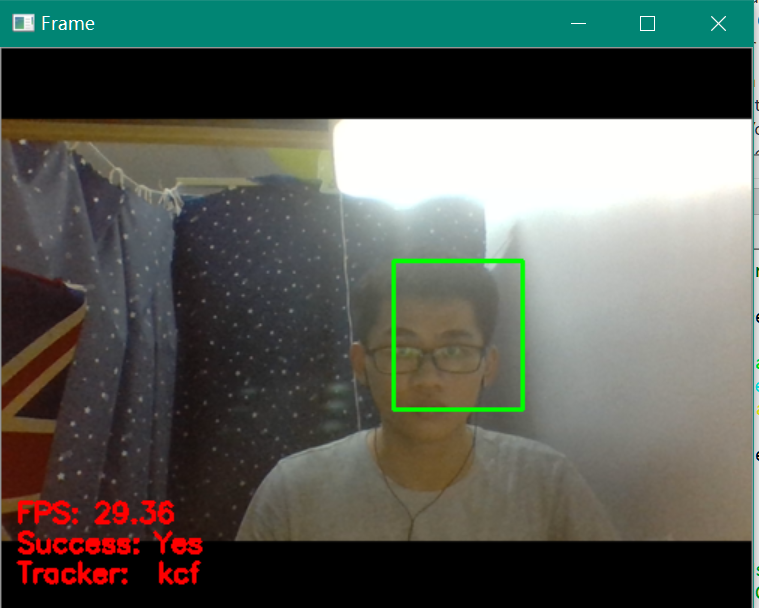
\includegraphics[width=0.8\linewidth]{1.png}
\end{center}
   \caption{识别棋子的结果}
\label{fig:long}
\label{fig:onecol}
\end{figure}

\subsection{识别方块}

从1/3的h开始,一条横线一条横线分析,遇到底色和阴影颜色都不相同的颜色时,进行统计分析。对每个X值求和及对该颜色的出现的次数记
录下
来。然后求出X的值的平均值,即为方块的所在中心的X坐标。对于方块中心的Y坐标,因为穿过左右顶点的线是有多条的,抓住这一特性,就可
以求Y
坐标。
\begin{figure}[t]
\begin{center}
%\fbox{\rule{0pt}{2in} \rule{0.9\linewidth}{0pt}}
   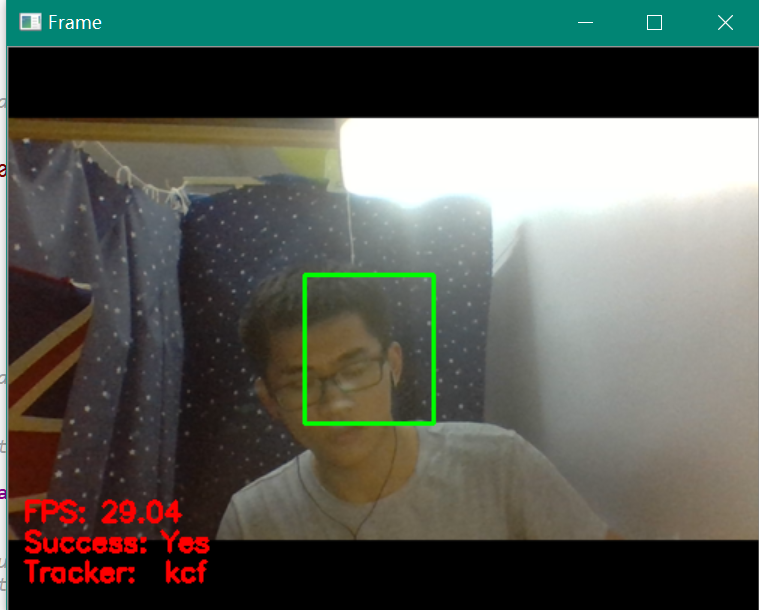
\includegraphics[width=0.8\linewidth]{2.png}
\end{center}
   \caption{识别方块的结果}
\label{fig:long}
\label{fig:onecol}
\end{figure}

\subsection{计算时间}
计算图中白线的距离,然后乘上一定的比列系数,即可得到按压的时间,然后让电脑输入命令,模拟按压就可以实现精准跳跃
\begin{figure}[t]
\begin{center}
%\fbox{\rule{0pt}{2in} \rule{0.9\linewidth}{0pt}}
   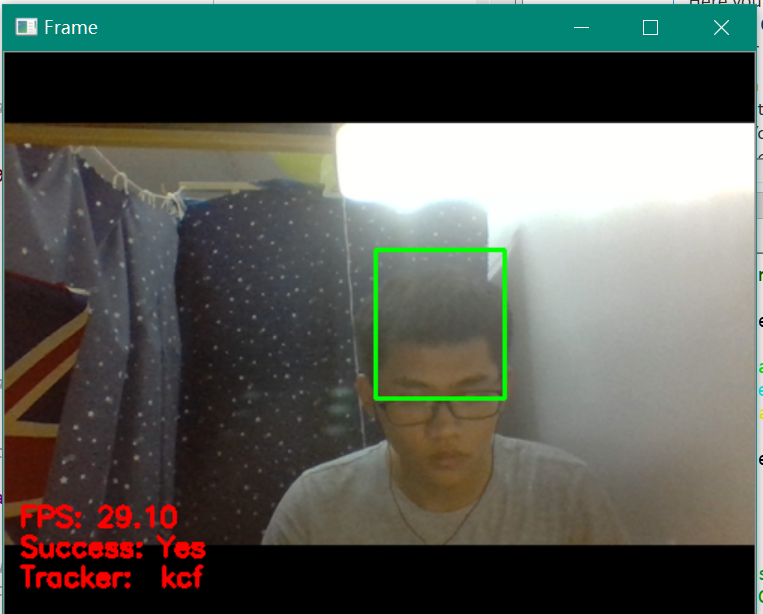
\includegraphics[width=0.8\linewidth]{3.png}
\end{center}
   \caption{计算时间的结果}
\label{fig:long}
\label{fig:onecol}
\end{figure}

%-------------------------------------------------------------------------
\subsection{结果分析}

该算法的时间和空间的复杂度都在是可以接受的,只是遇到一些特殊的情况可能会识别错误,但是大多数情况下都是准确的。识别的偏差不是很大,而且按压的时间是有范围的,所以理论上来说,是“死不了的”!












{\small
\bibliographystyle{ieee_fullname}
\bibliography{egbib}
}

\end{document}
